%!TEX root = ./template-skripsi.tex
%-------------------------------------------------------------------------------
%                            BAB III
%               			PEMBAHASAN
%-------------------------------------------------------------------------------

\chapter{HASIL DAN PEMBAHASAN}

Dalam penelitian ini tahapan yang akan dilakukan adalah seperti gambar di bawah ini

\begin{figure}[H]
	\centering
	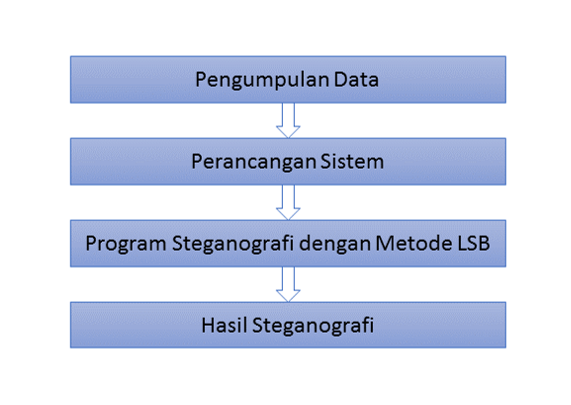
\includegraphics[width=0.8\textwidth]{gambar/alur_penelitian}
	\caption{Alur Penelitian}
	\label{alur_penelitian}
\end{figure}

\section{Pengumpulan Data}
\begin{enumerate}
	\item Studi Pustaka\\
	Penulis mendapatkan informasi yang berkaitan dengan steganografi melalui buku referensi dan juga dalam bentuk \emph{e-book}. Penulis juga mencari informasi melalui berbagai situs di internet yang sesuai dengan topik.	
	\item Studi Literatur\\
	Penulis mencoba mencari perbandingan dengan studi sejenis dari beberapa karya ilmiah lokal maupun internasional, seperti jurnal dan skripsi.	 
\end{enumerate}

\section{Perancangan Sistem}

	\subsection{Proses Penyisipan (\emph{Encoding}) pesan ke Citra \emph{Digital}}
	
	\begin{figure}[H]
		\centering
		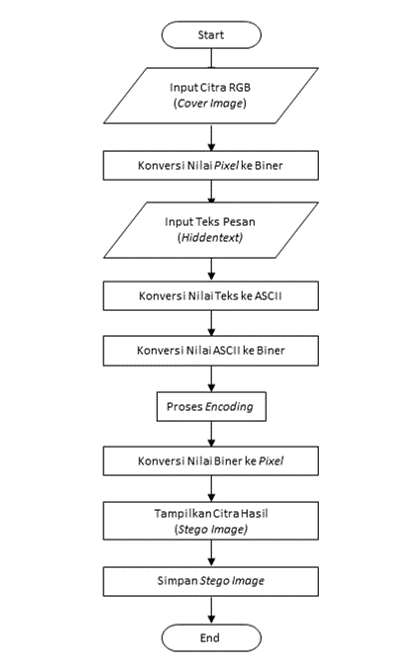
\includegraphics[height=0.8\textheight]{gambar/penyisipan3}
		\caption{\emph{Flowchart} Penyisipan Pesan Rahasia}
		\label{flowchart_penyisipan}
	\end{figure}

	Pada gambar di atas adalah \emph{flowchart} proses penyisipan pesan ke dalam \emph{file}
	citra (\emph{Cover Image}). Dimulai dengan membaca \emph{file} citra RGB. Untuk \emph{file} bitmap RGB maka setiap \emph{pixel} (titik) pada gambar tersebut terdiri dari susunan tiga warna \emph{Red, Green} dan \emph{Blue} yang masing-masing disusun oleh bilangan 8 bit (1 \emph{byte}) dari 0 sampai 255 atau dengan format biner 00000000 sampai 11111111. Setelah membaca \emph{pixel} dari \emph{file} citra langkah selanjutnya menentukan bit terkecil (LSB) pada \emph{Cover Image}.
	
	Selanjutnya adalah menyisipkan pesan (\emph{Hiddentext}) yang akan disembunyikan ke dalam \emph{Cover Image}. Pesan tersebut dikonversi terlebih dahulu menjadi nilai ASCII dan kemudian dikonversi kembali menjadi nilai Biner. Setelah itu terjadilah proses penyisipan (\emph{Encoding}). Selanjutnya biner yang telah disisipkan akan dikonversikan kembali ke dalam \emph{pixel}. Dan menyimpan citra yang telah disisipkan pesan ke dalam \emph{Cover Image} sehingga diperoleh atau	dapat ditampilkan sebuah gambar baru (\emph{Stego Image}).
	
	\subsection{Proses Ekstraksi (\emph{Decoding}) pesan dari Citra \emph{Digital}}
	
	\begin{figure}[H]
		\centering
		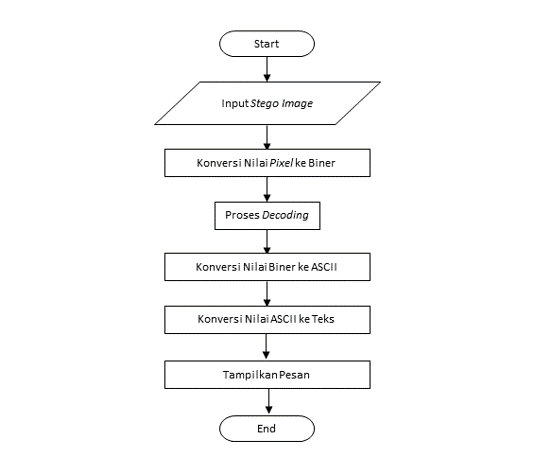
\includegraphics[height=0.6\textheight]{gambar/ekstraksi3}
		\caption{\emph{Flowchart} Ekstraksi Pesan Rahasia}
		\label{flowchart_ekstraksi}
	\end{figure}

	Pada gambar di atas adalah \emph{flowchart} proses ekstraksi pesan dari \emph{Stego Image} yang menghasilkan \emph{Hiddentext} yang terdapat di dalamnya. Prosesnya dimulai dengan membaca \emph{file} citra, dan mengubah \emph{pixel} ke dalam nilai biner. Kemudian proses ekstraksi (\emph{Decoding}). Setelah diperoleh bit-bit yang tersembunyi pada \emph{Cover Image} maka proses berikutnya adalah mengkonversi kembali pesan yang tersembunyi (\emph{Hiddentext}), sehingga pesan dapat ditampilkan kembali.

	\subsection{Desain Antar Muka Program}
	
	Berikut adalah GUI dari program steganografi yang dibangun dengan menggunakan Matlab.
	
	\begin{figure}[H]
		\centering
		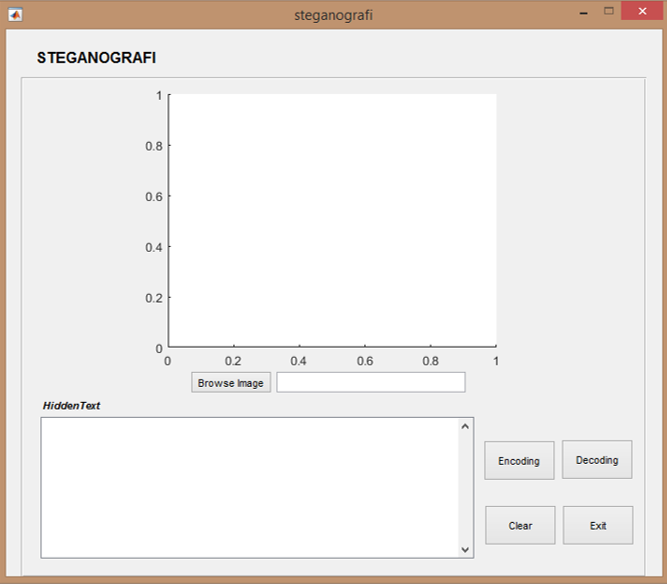
\includegraphics[width=1\textwidth]{gambar/mockup/1}
		\caption{GUI Steganografi}
		\label{desain_form}
	\end{figure}

	Dari tampilan tersebut, pengambilan gambar yang akan dijadikan sebagai \emph{Cover Image} dilakukan dengan menekan tombol "\emph{Browse Image}" dan gambar akan tampil. 
	
	\begin{figure}[H]
		\centering
		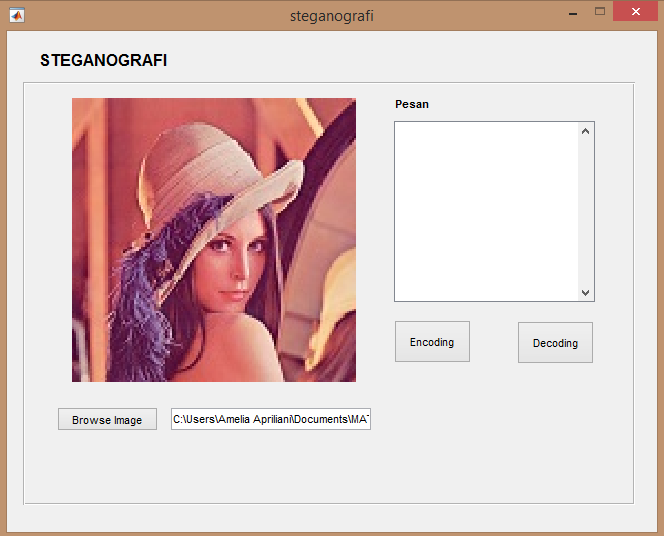
\includegraphics[width=1\textwidth]{gambar/mockup/2}
		\caption{GUI - \emph{Cover Image}}
		\label{desain_image}
	\end{figure}

	Setelah \emph{Cover Image} tampil maka pesan yang akan disisipkan atau \emph{Hiddentext} dapat dituliskan pada kolom pesan. Kemudian klik tombol \emph{Encoding} untuk melakukan proses \emph{Encoding}. Setelah proses \emph{Encoding}, maka akan didapatkan \emph{Stego Image} dan disimpan di dalam folder.
	
	\begin{figure}[H]
		\centering
		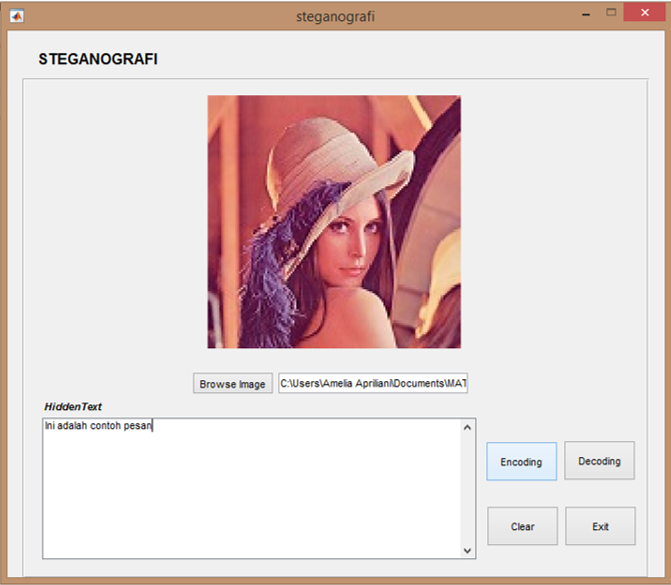
\includegraphics[width=1\textwidth]{gambar/mockup/3}
		\caption{GUI - Proses \emph{Encoding}}
		\label{desain_encoding}
	\end{figure}

	Jika ingin melakukan proses \emph{Decoding}, maka buka \emph{Stego Image} yang telah disimpan. Kemudian klik tombol \emph{Decoding} dan pesan akan didapatkan.

	\begin{figure}[H]
		\centering
		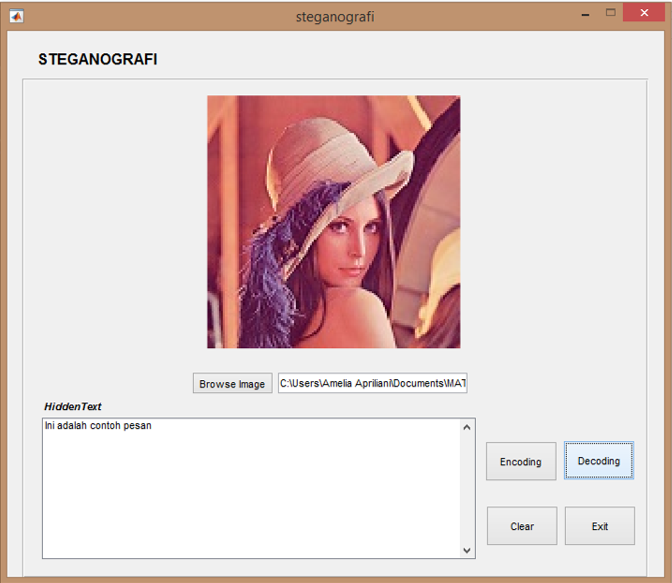
\includegraphics[width=1\textwidth]{gambar/mockup/5}
		\caption{GUI - Pesan Hasil \emph{Decoding}}
		\label{desain_pesan}
	\end{figure}

\section{Program Steganografi dengan Metode LSB}
Program diawali dengan pengambilan \emph{file} citra \emph{digital} yang akan digunakan, berikut adalah \emph{source code}-nya:
	\begin{figure}[H]
		\centering
		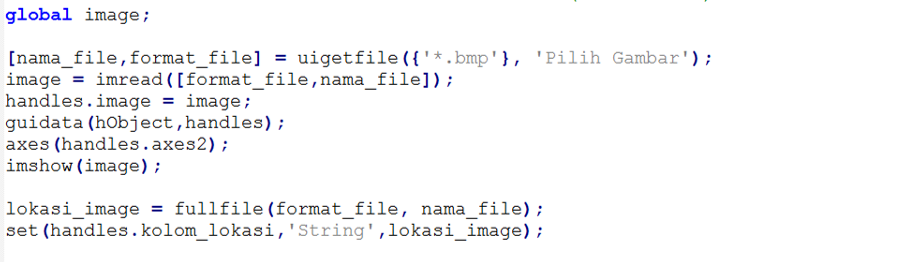
\includegraphics[width=1\textwidth]{gambar/sourcecode/browse_image}
		\caption{\emph{Source Code} - \emph{Browse Image}}
		\label{browse_image}
	\end{figure}

Selanjutnya adalah memasukkan pesan atau \emph{Hiddentext}. \emph{Hiddentext} yang akan dimasukkan tidak boleh melebihi batas maksimal karakter. Panjang karakter maksimal disesuaikan dengan besar \emph{pixel} pada \emph{file} citra. Panjang karakter maksimal dapat dihitung, berikut adalah \emph{source code}-nya:
	\begin{figure}[H]
		\centering
		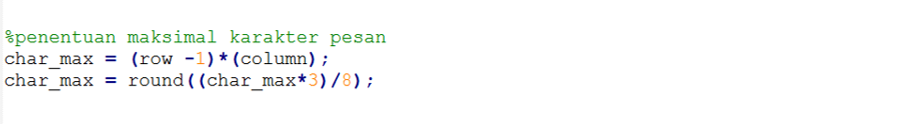
\includegraphics[width=1\textwidth]{gambar/sourcecode/karakter_maksimal}
		\caption{\emph{Source Code} - Menghitung Karakter Maksimal}
		\label{karakter_max}
	\end{figure}

Sedangkan untuk menghitung panjang \emph{hiddentext} yang telah dimasukkan adalah sebagai berikut:
	\begin{figure}[H]
		\centering
		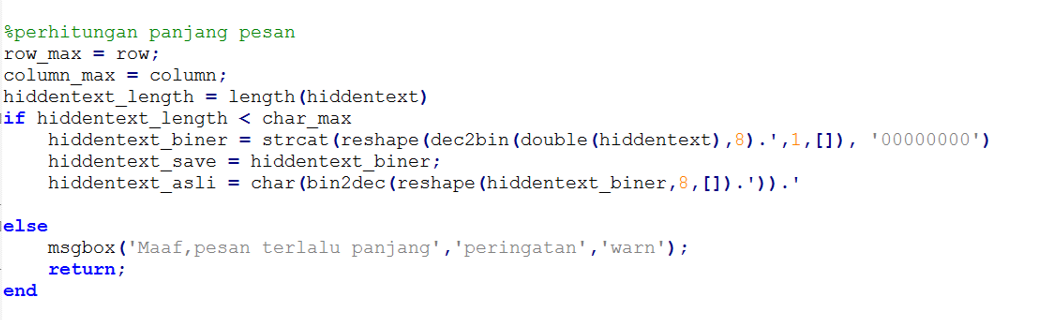
\includegraphics[width=1\textwidth]{gambar/sourcecode/panjang_pesan}
		\caption{\emph{Source Code} - Menghitung Panjang \emph{Hiddentext} yang Dimasukkan}
		\label{panjang_pesan}
	\end{figure}

\subsection{\emph{Encoding}}
Pada tugas akhir ini metode yang digunakan dalam steganografi adalah metode LSB. Proses \emph{Encoding} merupakan proses penyisipan pesan atau \emph{Hiddentext} ke dalam \emph{file} citra. Berikut adalah cuplikan \emph{source code} proses \emph{Encoding} dengan menggunakan metode LSB:
	\begin{figure}[H]
		\centering
		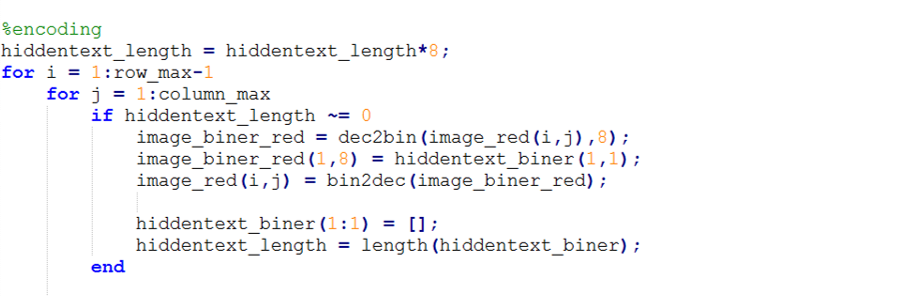
\includegraphics[width=1\textwidth]{gambar/sourcecode/cuplikan_encoding}
		\caption{\emph{Source Code} - Cuplikan \emph{Encoding}}
		\label{cuplikan_encoding}
	\end{figure}

\subsection{\emph{Decoding}}
Proses \emph{Decoding} merupakan proses pengambilan kembali pesan atau \emph{Hiddentext} yang telah disisipkan ke dalam \emph{file} citra. Berikut merupakan cuplikan dari \emph{source code} proses \emph{Decoding}:
	\begin{figure}[H]
		\centering
		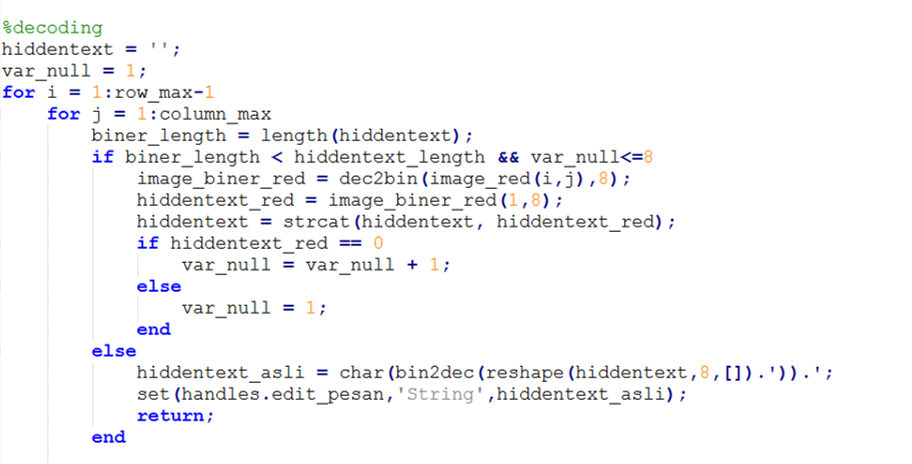
\includegraphics[width=1\textwidth]{gambar/sourcecode/cuplikan_decoding}
		\caption{\emph{Source Code} - Cuplikan \emph{Decoding}}
		\label{cuplikan_decoding}
	\end{figure}
	
\section{Hasil Steganografi}
Setelah dilakukan pengujian terhadap program Steganografi, maka didapatkan hasil sebagai berikut:
	\subsection{Pengujian Berdasarkan Bit pada \emph{File} Citra}
	Pengujian ini menguji berapakah batas Bit \emph{File} Citra yang bisa dimasukkan di dalam program.
	
	%masukkin table
	\begin{table}[H]
		\centering
		\caption{Bit pada \emph{File} Citra}
		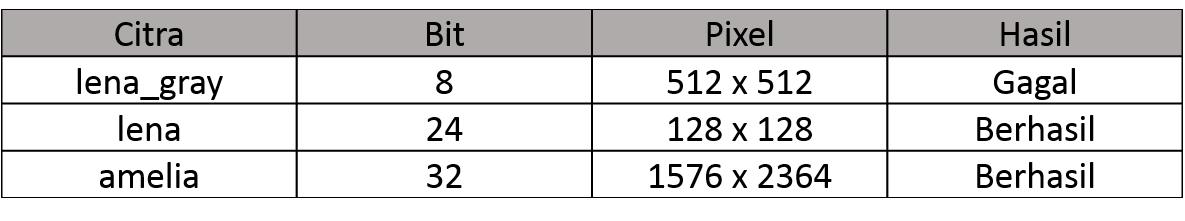
\includegraphics[width=1.0\textwidth]{gambar/table_bitcitra}
		\label{tabel_bitcitra}
	\end{table}
	
	Pada tabel tersebut terlihat bahwa \emph{file} citra dengan ukuran 8 bit tidak berhasil untuk disisipkan pesan karena tidak mengandung komponen RGB. Sedangkan untuk \emph{file} citra 24 dan 32 bit bisa digunakan sebagai \emph{Cover Image} untuk menyisipkan pesan karena mengandung komponen RGB didalamnya.
	
	\begin{figure}[H]
		\centering
		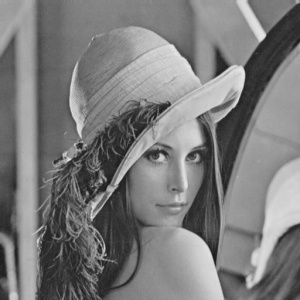
\includegraphics[width=0.4\textwidth]{gambar/matlab/lena_gray}
		\caption{\emph{File} Citra 8 Bit}
		\label{lena_gray8}
	\end{figure}
	
	\begin{figure}[H]
		\centering
		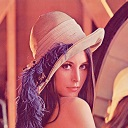
\includegraphics[width=0.4\textwidth]{gambar/matlab/lena}
		\caption{\emph{File} Citra 24 Bit}
		\label{lena24}
	\end{figure}

	\begin{figure}[H]
		\centering
		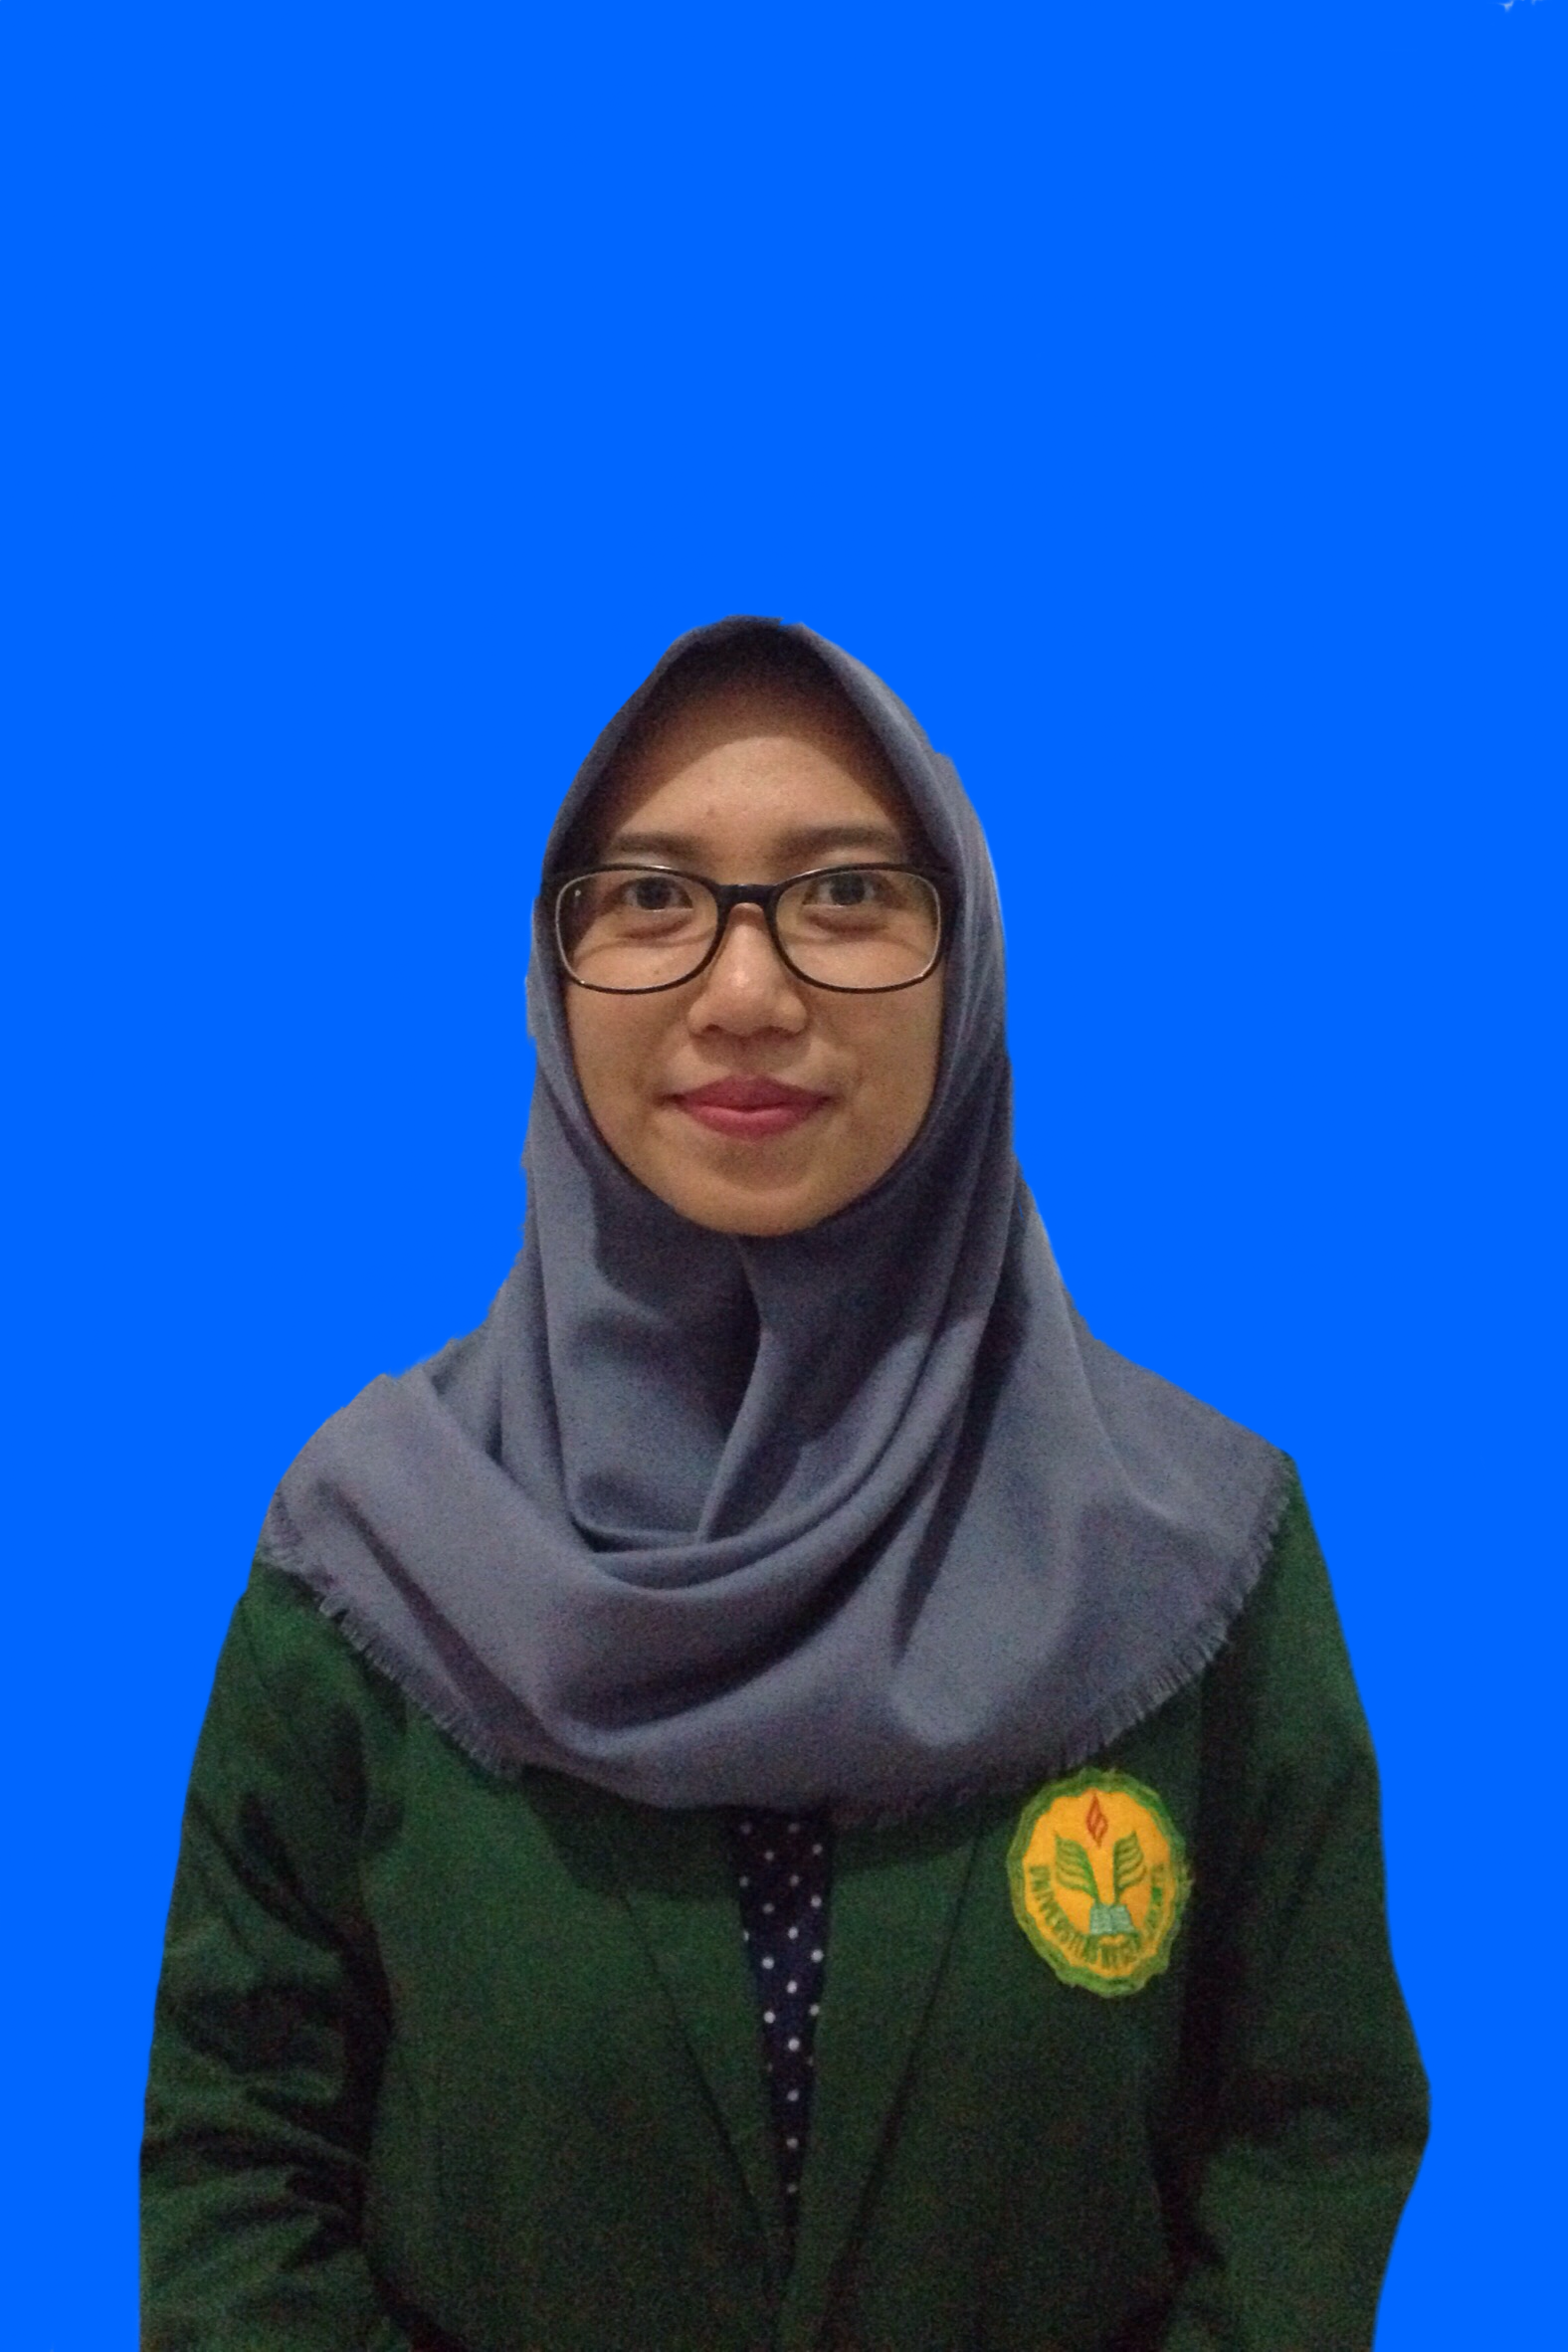
\includegraphics[width=0.4\textwidth]{gambar/matlab/amelia}
		\caption{\emph{File} Citra 32 Bit}
		\label{amelia32}
	\end{figure}

	\subsection{Pengujian Berdasarkan \emph{Imperceptible}}
	Pengujian ini menguji kualitas citra \emph{digital}, apakah citra \emph{digital} akan mengalami perubahan yang mencurigakan atau tidak secara visual. Pengujian ini dikatakan berhasil apabila kualitas dari \emph{Stego Image} yang dihasilkan tidak berbeda jika dibandingkan dengan berkas aslinya atau \emph{Cover Image}.

	%gambar cover
	\begin{figure}[H]
		\centering
		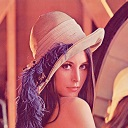
\includegraphics[width=0.4\textwidth]{gambar/matlab/lena}
		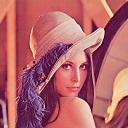
\includegraphics[width=0.4\textwidth]{gambar/matlab/lena_kalimat}
		\caption{Perbandingan \emph{File} Citra - lena.bmp}
		\label{lena_stego}
	\end{figure}

	%gambar cover
	\begin{figure}[H]
		\centering
		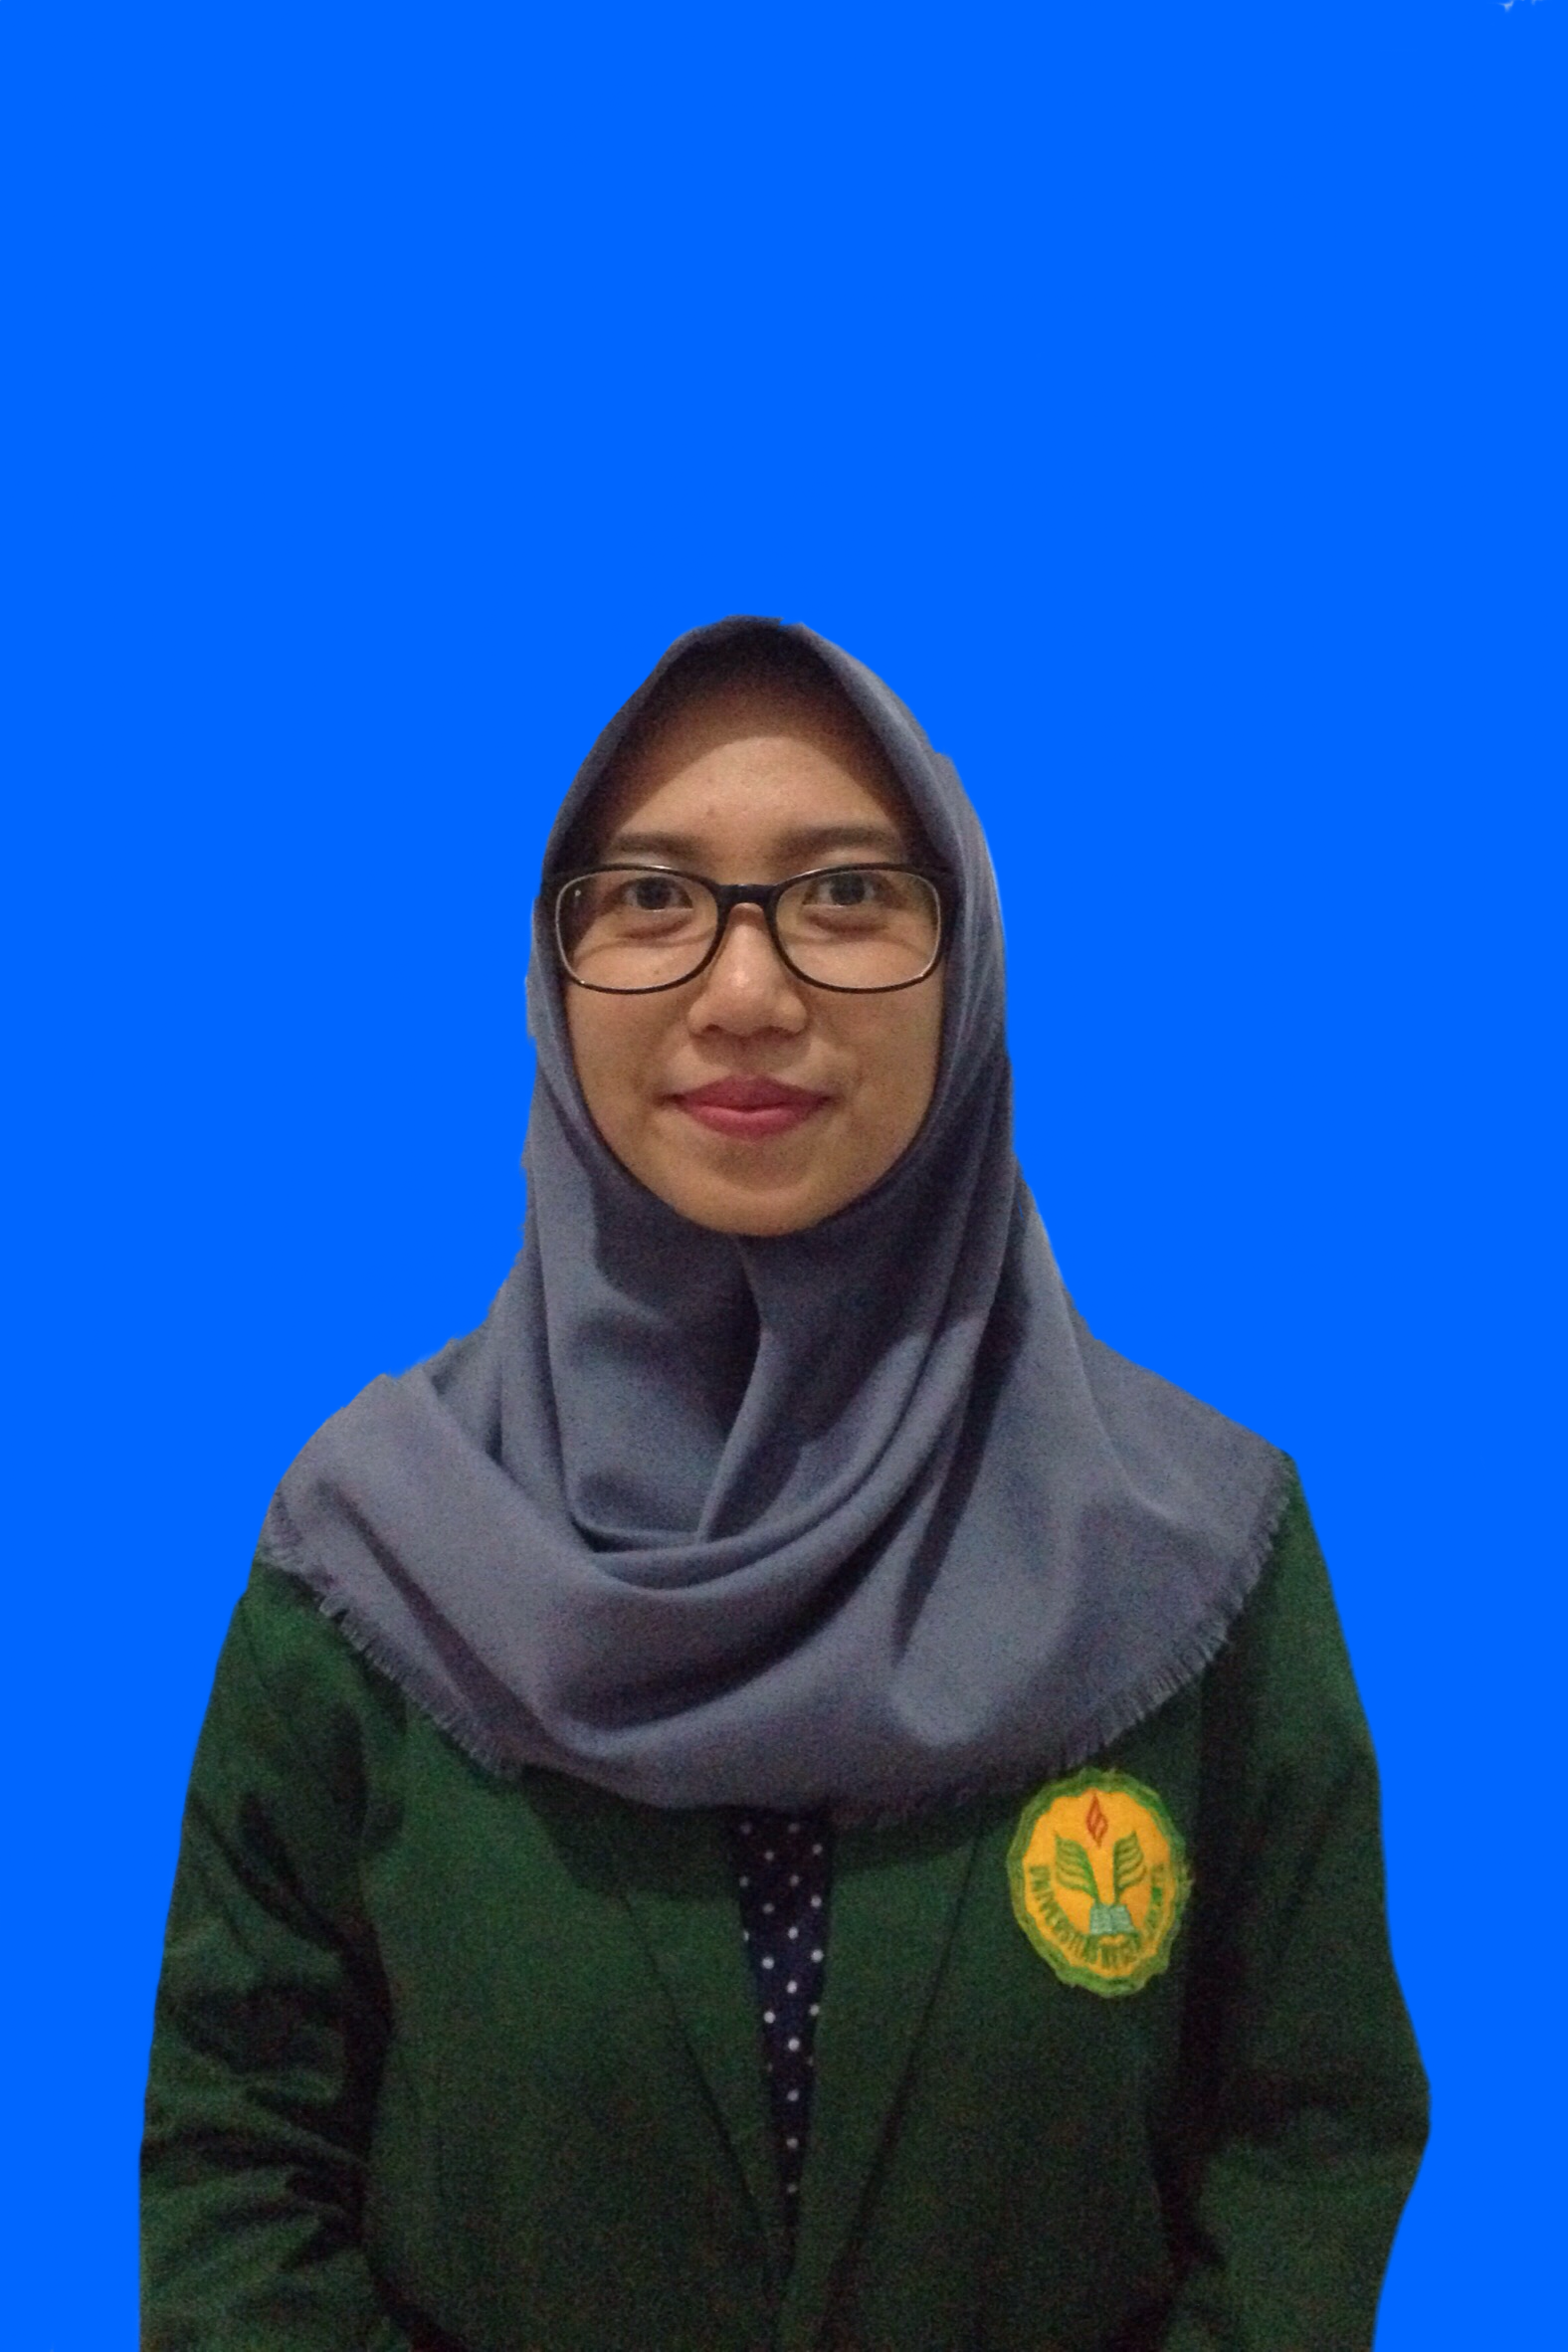
\includegraphics[width=0.4\textwidth]{gambar/matlab/amelia}
		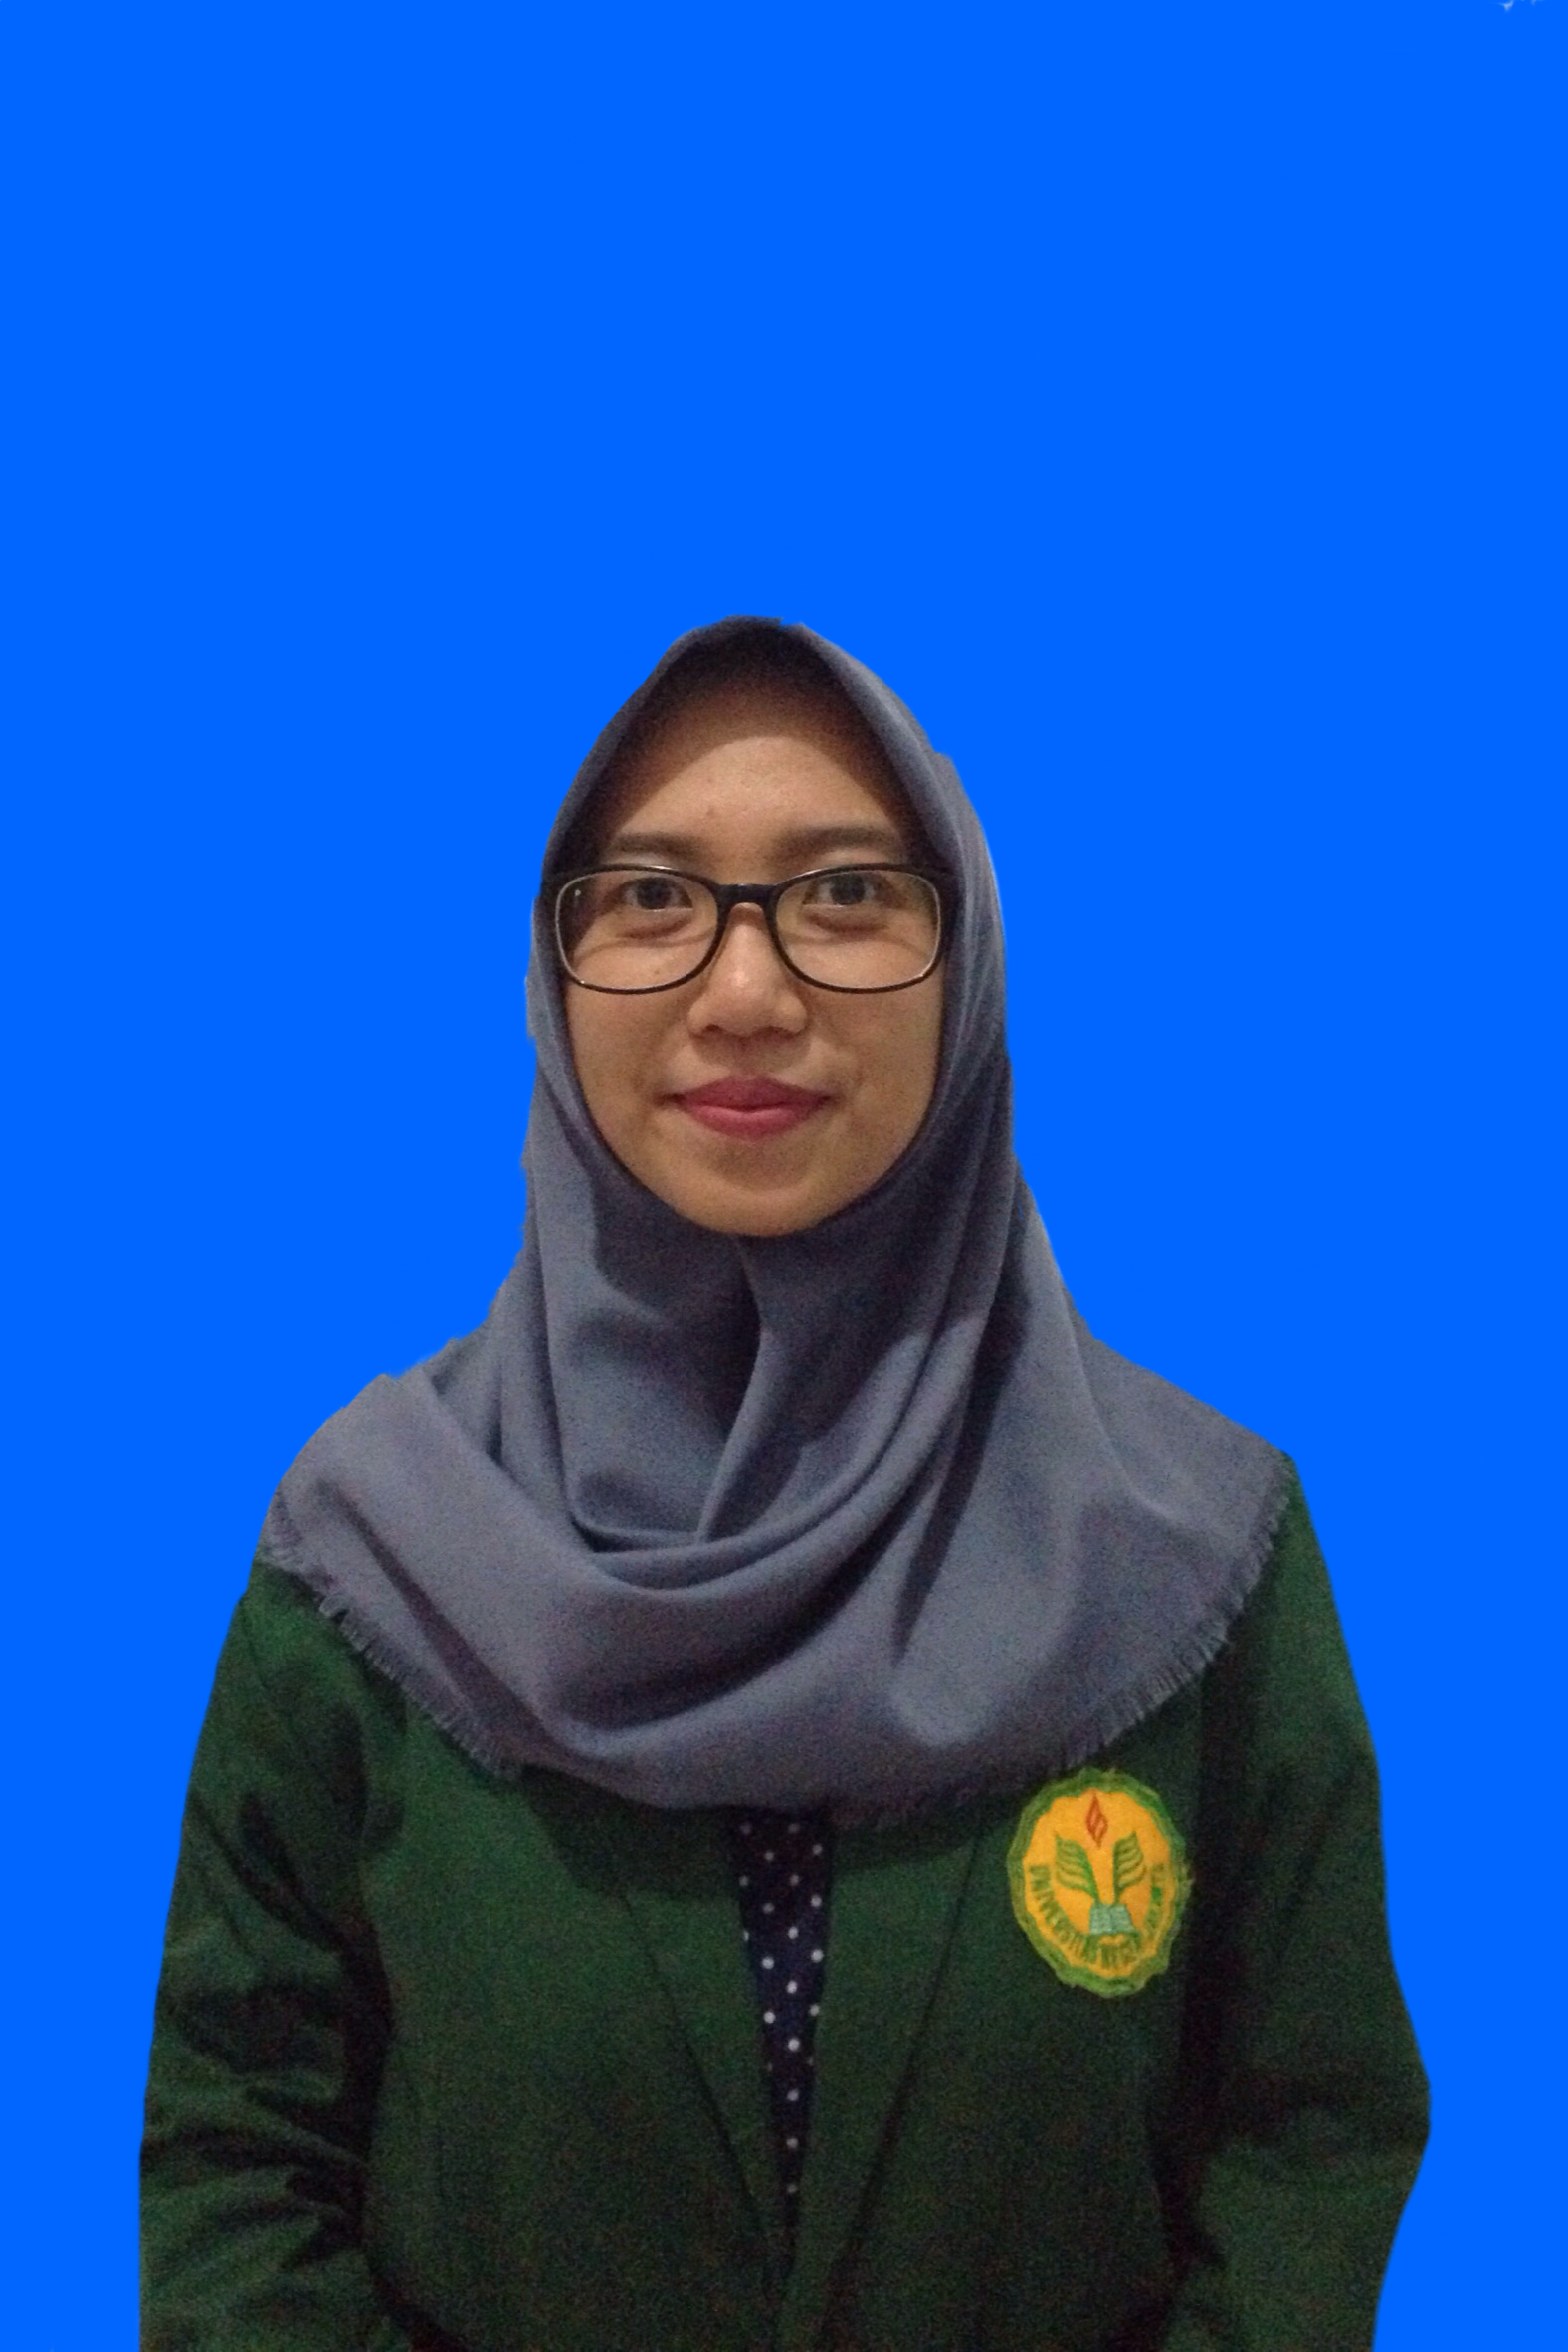
\includegraphics[width=0.4\textwidth]{gambar/matlab/amelia_kalimat}
		\caption{Perbandingan \emph{File} Citra - amelia.bmp}
		\label{amelia_stego}		
	\end{figure}


	Pada gambar 3.16 dan 3.17 menunjukkan jika dibandingkan secara visual maka tidak tampak perubahan yang terjadi dari \emph{Cover Image} ke \emph{Stego Image}. Tidak tampak perubahan warna ataupun bentuk dari \emph{Cover Image}.

	\subsection{Pengujian Berdasarkan \emph{Fidelity}}
	Pengujian ini berdasarkan proses penyembunyiaan pesan atau \emph{Encoding}. Pada proses penyembunyian pesan dapat berhasil apabila ukuran pesan yang akan disembunyikan sesuai dengan kapasitas \emph{file} citra. Apabila ukuran pesan melebihi kapasitas maksimal dari \emph{file} citra, maka program tidak akan melanjutkan proses \emph{Encoding}. Kapasitas pesan dipengaruhi oleh ukuran \emph{pixel} dari citra \emph{digital}. Semakin besar ukuran \emph{pixel} dari citra \emph{digital}, maka semakin besar pula kapasitas pesan yang bisa disembunyikan.
	
	%masukkin tabel
	\begin{table}[H]
		\centering
		\caption{Karakter Maksimal Pesan pada \emph{File} Citra}
		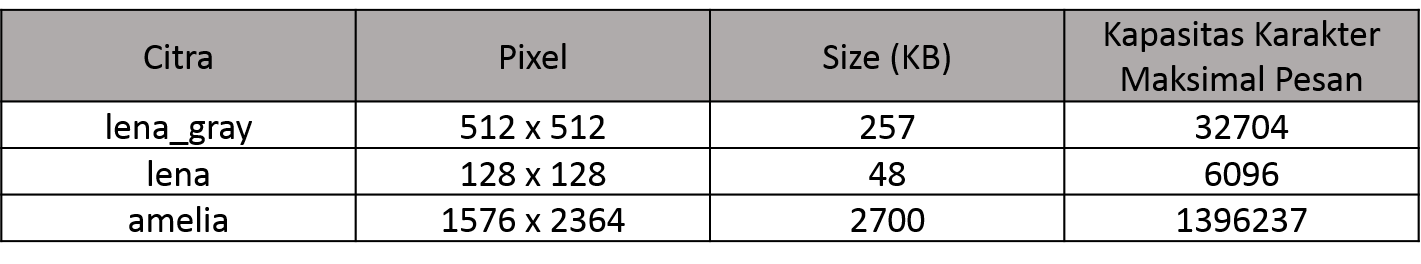
\includegraphics[width=1.0\textwidth]{gambar/table_karaktermax3}
		\label{tabel_karaktermax2}
	\end{table}

	\begin{table}[H]
		\centering
		\caption{Hasil Proses \emph{Encoding}}
		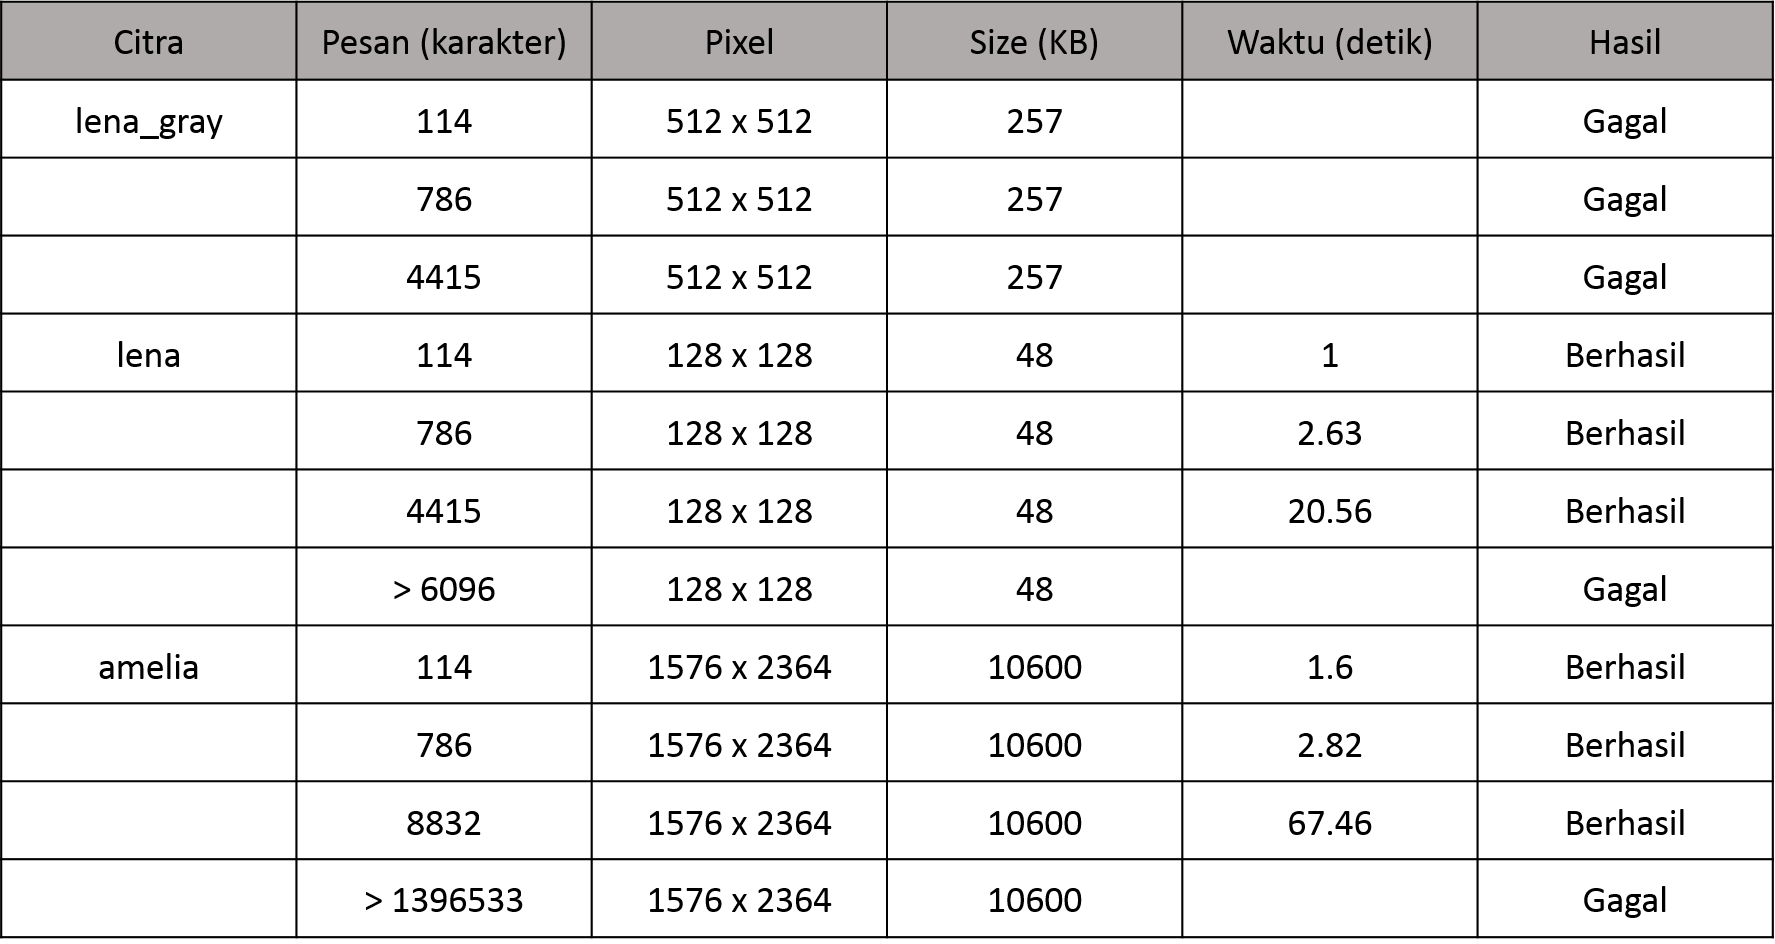
\includegraphics[width=1.0\textwidth]{gambar/table_hasilencode3}
		\label{tabel_hasilencode3}
	\end{table}

	Pada tabel di atas terlihat data \emph{file} citra yang dimasukkan adalah 24 bit dan 32 bit. Setiap  \emph{file} citra dimasukkan pesan atau \emph{Hiddentext} dengan beragam panjang karakter. Panjang dari karakter pesan berpengaruh terhadap kecepatan dalam proses \emph{Encoding}. Semakin panjang karakter yang dimasukkan, maka semakin lama juga waktu yg dibutuhkan. Untuk \emph{file} citra $lena_ gray$ tidak bisa dilakukan proses \emph{Encoding}, karena \emph{file} tersebut adalah \emph{file} 8 bit. Pada \emph{file} citra lena dan amelia, berhasil dilakukan proses \emph{Encoding}, kecuali ketika panjang karakter pesan melebihi kapasitas maksimal dari \emph{file} citra tersebut.

	\subsection{Pengujian Berdasarkan \emph{Recovery}}
	Pengujian ini berdasarkan proses ektraksi pesan atau \emph{Decoding}. Untuk membuktikan apakah program steganografi ini berhasil, maka harus dapat dibuktikan bahwa pesan di dalam \emph{Stego Image} dapat diambil kembali. Jika pengujian dilakukan dengan benar, maka \emph{Hiddentext} dapat ditampilkan sesuai dengan yang dimasukkan. 
	
	Pada penelitian ini, pesan yang dihasilkan dari proses \emph{Decoding} tidak menghasilkan karakter-karakter aneh yang tidak dapat dibaca. Hasil dari pengujian ekstraksi pesan dapat dilihat pada tabel 3.2
	 
	%masukkin tabel
	\begin{table}[H]
		\centering
		\caption{Hasil Proses \emph{Decoding}}
		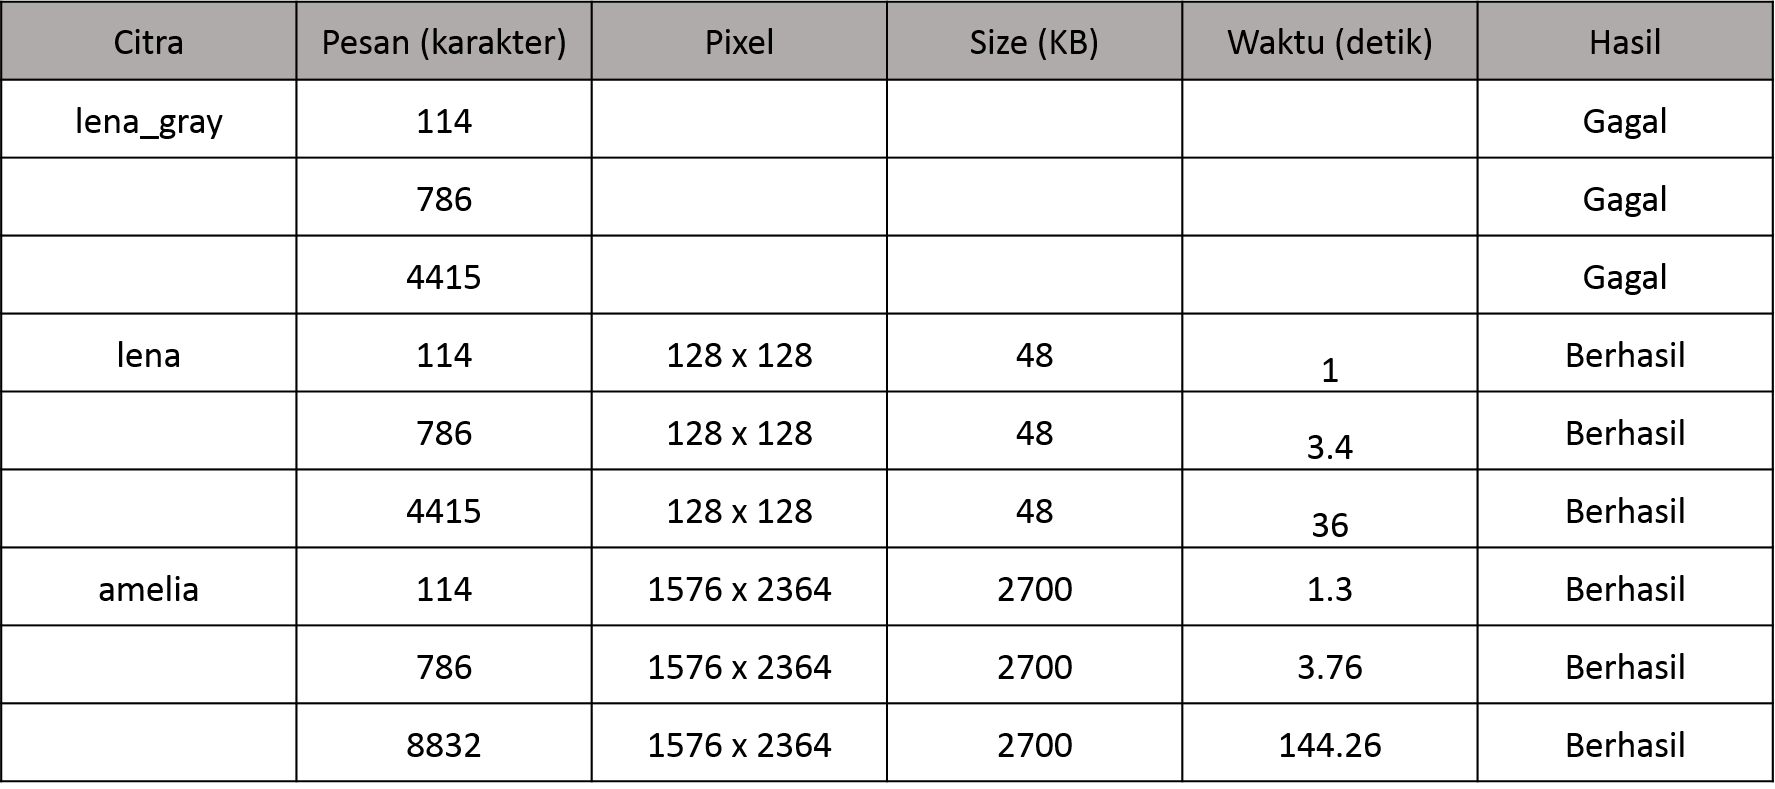
\includegraphics[width=1.0\textwidth]{gambar/table_hasildecode3}
		\label{tabel_hasildecode3}
	\end{table}
	
	Pada proses \emph{Decoding}, besar \emph{pixel} dan ukuran pada \emph{Stego Image}, tidak mengalami perubahan. Hal ini tidak akan memberikan kecurigaan terhadap \emph{file} citra. Waktu yang dibutuhkan dalam proses \emph{Decoding} juga berbanding lurus dengan panjang karakter pesan. Semakin banyak karakter pesan atau \emph{Hiddentext} yang dimasukkan, maka semakin lama waktu yang dibutuhkan. Pada proses \emph{Decoding} terhadap kedua \emph{file} citra hasilnya adalah berhasil. Karena pesan yang ada pada \emph{file} citra tersebut bisa ditampilkan kembali.
	
	Pada pengujian ini juga dilakukan teknik \emph{cropping} pada beberapa \emph{Stego Image}. Setelah dilakukan \emph{cropping}, \emph{Stego Image} tersebut tidak berhasil untuk menampilkan pesan asli yang ada di dalamnya, hanya karakter-karakter aneh yang ditampilkan. 
	
	\begin{table}[H]
		\centering
		\caption{Hasil Proses \emph{Cropping} }
		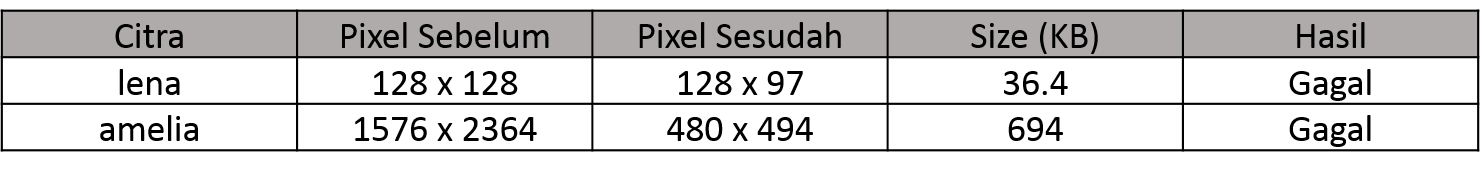
\includegraphics[width=1.0\textwidth]{gambar/table_cropping}
		\label{tabel_cropping}
	\end{table}

	\begin{figure}[H]
		\centering
		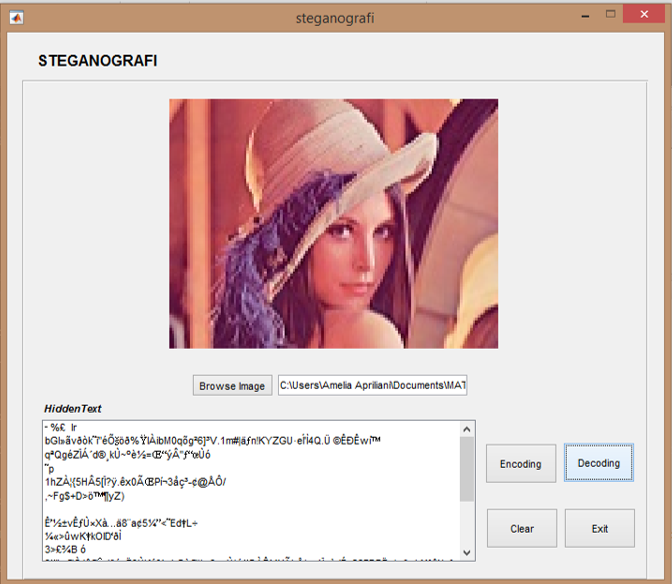
\includegraphics[width=0.8\textwidth]{gambar/matlab/lena_crop}
		\caption{\emph{File} Citra lena.bmp Hasil \emph{Cropping}}
		\label{lena_crop}
	\end{figure}

	\begin{figure}[H]
		\centering
		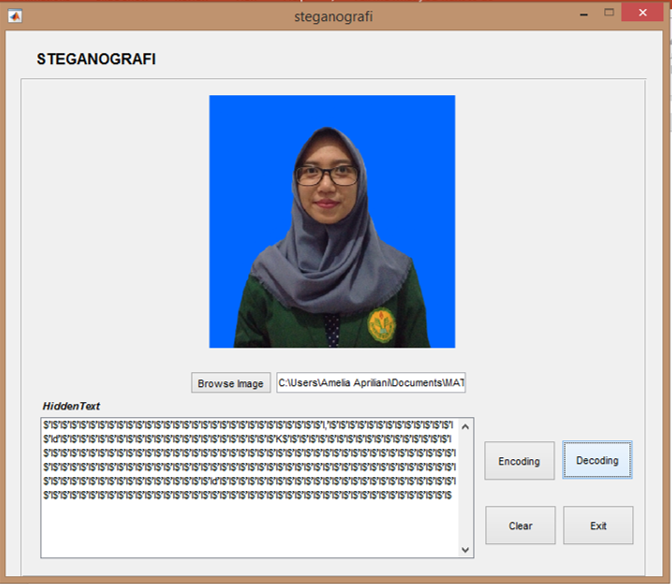
\includegraphics[width=0.8\textwidth]{gambar/matlab/amelia_crop}
		\caption{\emph{File} Citra amelia.bmp Hasil \emph{Cropping}}
		\label{amelia_crop}
	\end{figure}

	Teknik \emph{cropping} dapat menyebabkan \emph{pixel-pixel} pada \emph{file} citra menjadi hilang. Sehingga pesan yang sudah disisipkan di dalam \emph{file} citra tersebut tidak dapat ditampilkan kembali.
		 
	\subsection{Kesimpulan Pengujian}
	Dari pengujian di atas dapat disimpulkan bahwa program steganografi yang dibuat ini menghasilkan hasil yang cukup baik untuk setiap penyembunyian pesan ke dalam \emph{file} citra. Pemilihan \emph{Cover Image} yang akan digunakan dan panjang karakter pesan yang akan dimasukkan sangat berpengaruh, karena semakin besar ukuran \emph{file} citra yang digunakan dan semakin sedikit karakter yang disisipkan pada \emph{file} citra maka semakin sedikit perubahan yang terjadi setelah proses penyisipan pada \emph{file} citra atau kualitas sebelum penyisipan dan setelah penyisipan tidak berpengaruh banyak pada perubahan kualitas citra sebelumnya.
	